\documentclass[../main.tex]{subfiles}
\begin{document}

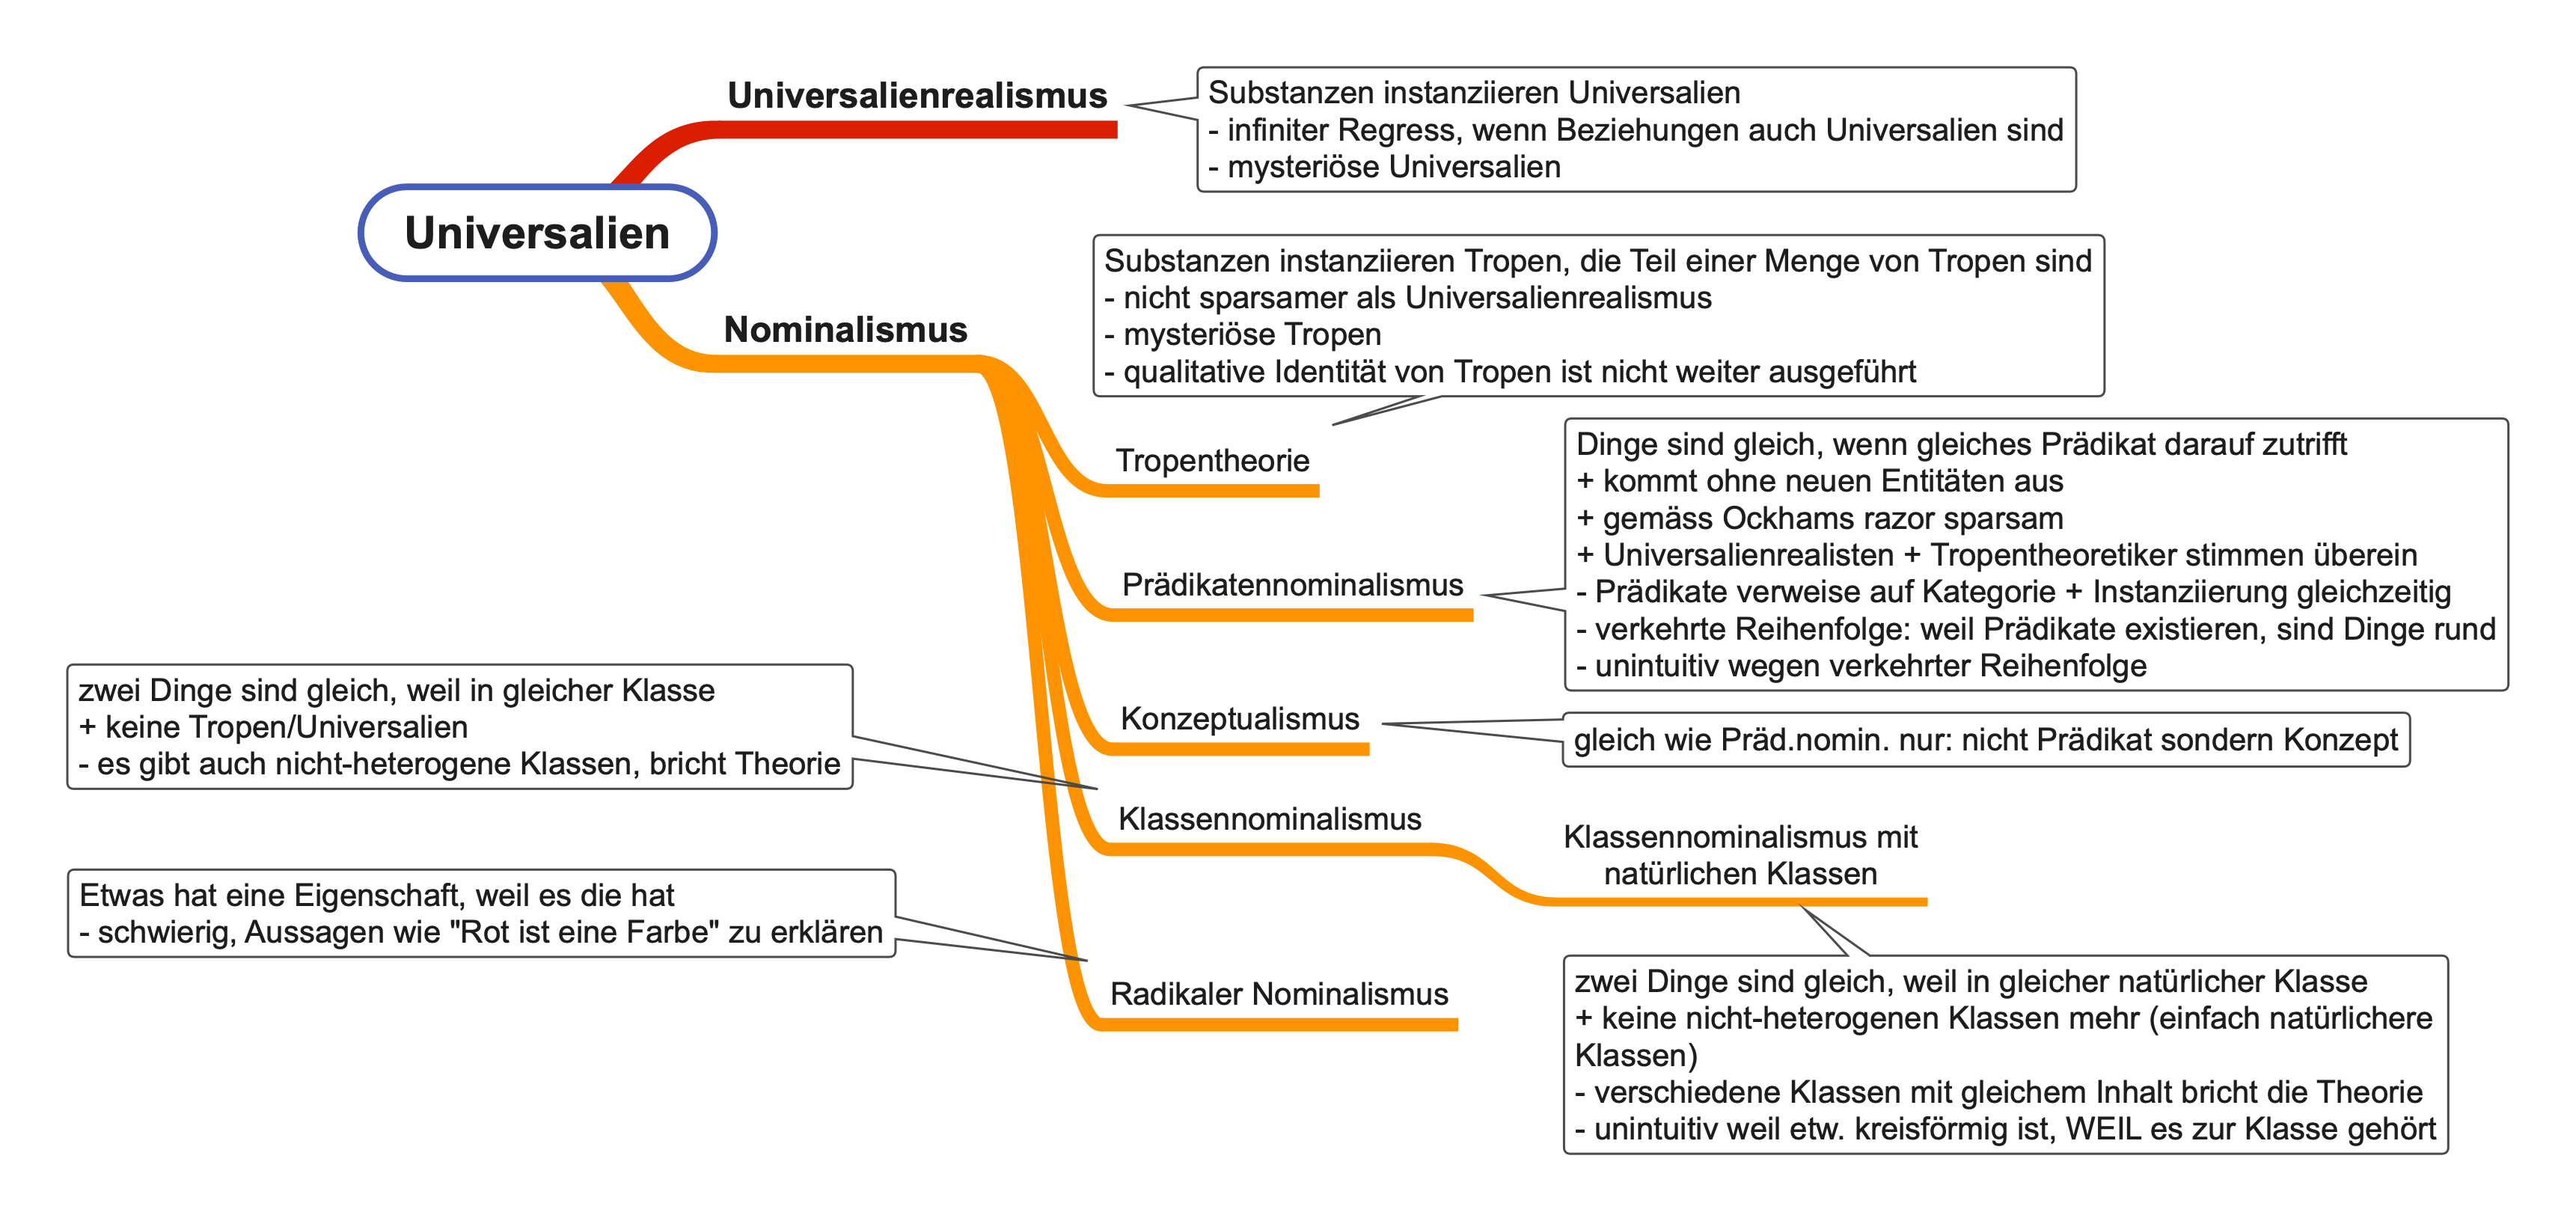
\includegraphics[width=\textwidth]{images/Universalien_Uebersicht.png}

\section{Was ist Metaphysik} 
<<Universalien vs Nominalismus>> sind der Metaphysik unterzuordnen. Diese wurde bereits von Aristoteles begründet und dreht sich um die Frage des \textit{Seins} und um \textit{das Seiende} im Allgemeinen, den Begriff der Substanz, Möglichkeit und Wirklichkeit, den \textit{unbewegten Beweger} (Ursache für den Ablauf des Universums) und vielem mehr. Später wurde die Metaphysik etwas umgedeutet als eigene Disziplin und sollte der Frage hintergehen, was \textit{hinter der Physik} liegt	. 

\subsection{Allgemeine Metaphysik}
Unter der allgemeinen Metaphysik oder <<Metaphysik im engeren Sinne>> versteht man die \textit{Ontologie}. Ihre zentralen Fragen sind:
\begin{itemize}
	\item Welche Arten von Dingen gibt es (Eigenschaften, Zahlen, Mengen, Ereignisse, Tatsachen, usw.)?
	\item Was ist die Natur dieser Dinge und wie stehen sie zueinander in Beziehung?
	\item Was ist Existenz? Was bedeutet es zu sagen, dass etwas existiert (heute \textit{Metaontologie})?
\end{itemize}

\subsection{Spezielle Metaphysik}
Die spezielle Metaphysik, auch <<Metaphysik im weiteren Sinne>>, behandelt folgende Themen:
\begin{itemize}
	\item Gibt es Gott? Was ist seine Natur (\textit{rationale Theologie})?
	\item In welchem Verhältnis steht der Geist zum Körper? Wie stehen geistige Eigenschaften zu körperlichen/physischen Eigenschaften? Was ist personale Identität (\textit{rationale Psychologie})?
	\item Hat das Universum einen Anfang in der Zeit? Gibt es eine Ursache für die Entstehung des Universum (\textit{rationale Kosmologie})?
\end{itemize}

\section{Problem der Universalien}
{\centering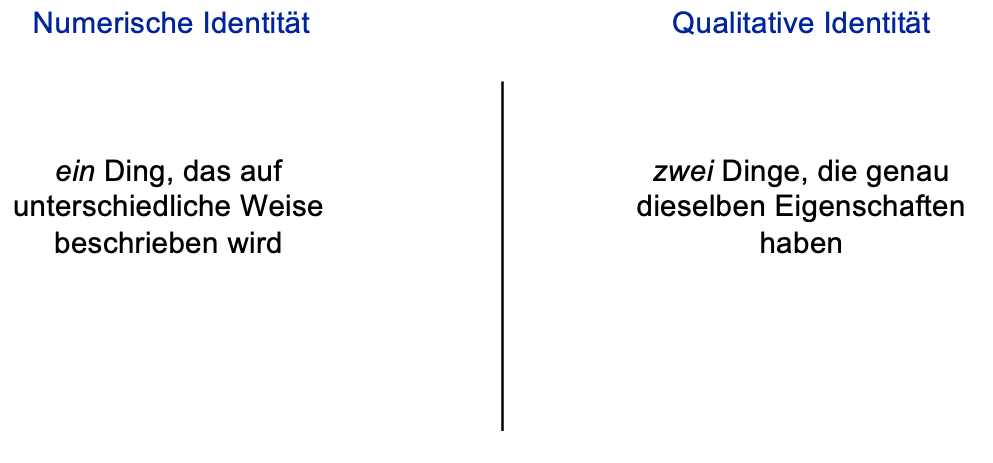
\includegraphics[height=5cm]{images/numerische_und_qualitative_identitaet.png}\endcenter}
Das Problem der Universalien ist ähnlich wie dieses, das im Teil der Personalen Identität (\ref{SectionPersonaleIdentitaet}) angesprochen wird; Was ist dafür verantwortlich, dass zwei numerisch verschiedene Dinge in einer oder mehreren Hinsichten gleich (qualitativ identisch) sind? Was macht zum Beispiel zwei gleiche Wörter identisch? Dass sie beide Wörter sind? Dass sie beide gleich viele Buchstaben in der gleichen Reihenfolge haben? Oder dass sie zum gleichen Typ gehören? Damit lässt sich eine zweite Version des Problems aufbauen: Was ist dafür verantwortlich, dass zwei verschiedene Dinge zum gleichen Typ gehören?

In anderen Worten lässt sich das Universalienproblem so ausdrücken: Bezieht sich das <<etwas sein>> wie in <<das Blatt ist rot>> auf ein Ding, das gegeben ist?

\section{Der Universalienrealismus}
Der Universalienrealismus (Bertrand Russel, D. M. Armstrong, u.a.) erklärt die Zugehörigkeit zweier Dinge zum gleichen Typ mit deren Instanzierung der gleichen Eigenschaft (exemplifizieren). Als Beispiel dafür nimmt man zwei Kreise. Beide sind eigenständig, also haben ihre eigene numerische Identität. Sie sind jedoch qualitativ gleich, weil sie beide die Eigenschaft <<Kreisförmigkeit>> instanziieren. 

\subsection{Klassischer Universalienrealismus}
\paragraph{These} 
\begin{enumerate}[label=(\alph*)]
	\item Es gibt nicht instanziierbare \textit{Substanzen} ( = Einzeldinge), die Eigenschaften instanziieren.
	\item Es gibt \textit{Universalien} ( = Eigenschaften), die von mehreren Dingen instanziiert werden können. 
	\item Dass zwei \textit{Substanzen} in einer Hinsicht gleich (qualitativ identisch) sind, kann dadurch erklärt werden, dass sie dasselbe Universale instanziieren. 
	\item Eine Substanz kann mehrere Universalien instanzieren.
\end{enumerate} 
\paragraph{Erklärung} Der klassische Universalienrealismus betrachtet alle Gegenstände als Substanzen, die ihre Eigenschaft auf ihre Beziehung zu einer oder mehreren Universalien zurückführen. Oder anders ausgedrückt: Die Substanz instanziiert eine oder mehrere Universalien. Durch diese Instanziierung können Substanzen miteinander qualitativ verglichen werden. Sind beide qualitativ gleich, so sind deren Universalen \textit{numerisch} identisch (sie haben das gleiche Universal).

{\centering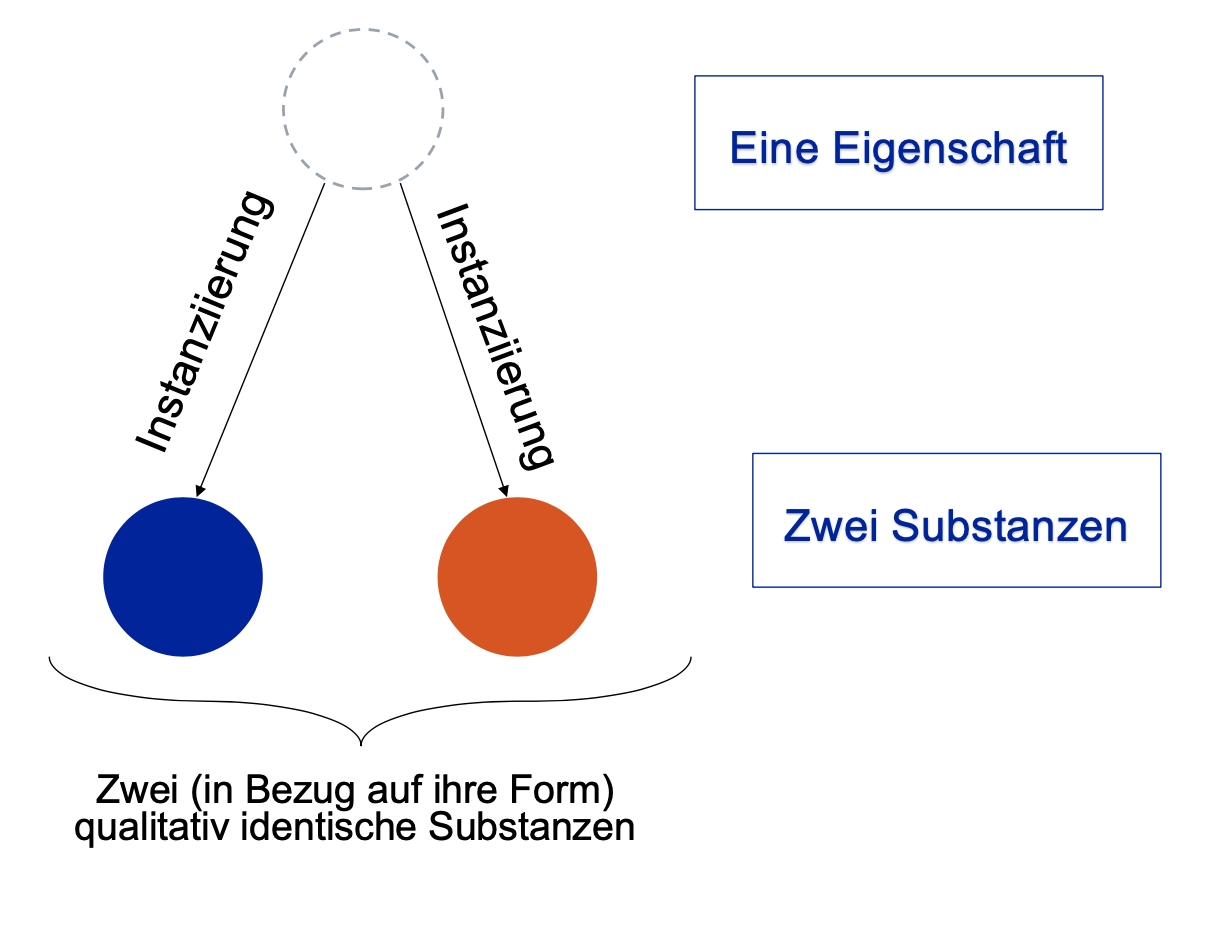
\includegraphics[height=7cm]{images/eine_eigenschaft_zwei_substanzen_universalienrealismus.png}\endcenter}

Sind zwei Gegenstandspaare jeweils einen Meter von ihrem Gegenstück entfernt, so instanziieren beide Paare, nennen wir sie Paar<A,B> und Paar<C,D>, dasselbe Universal <<Einen-Meter-Entfernt-Sein>>. Es instanziieren jedoch nicht A oder C das <<Einen-Meter-Entfernt-Sein>>-Universal, sondern die Relation zwischen A und B, resp. zwischen C und D. Gemäss dem Universalienrealismus gehören auch diese Relationen zu den Universalien, nicht nur Eigenschaften. Dabei werden die Relationen noch in ihrer \textit{Stelligkeit} unterschieden; Es gibt zweistellige Relationen (A ist einen Meter von B entfernt) die Tupel genannt werden, dreistellige (A befindet sich zwischen B und C), Tripel genannt, und allgemein n-stellige Relationen (n-Tupel).

\paragraph{Probleme} 
\begin{enumerate}
	\item Das Problem des infiniten Regresses: Nimmt man zwei Substanzen A und B, die jeweils von ein anderen Universal instanziieren und betrachtet man diese als Paare (wie oben erklärt) Paar<A,Universal von A> und Paar<B, Universal von B>, so sind diese Paare zumindest in der Hinsicht identisch, dass sie beide Paare sind. Um dies in der Universalientheorie abzubilden, müsste also das Paar<A, Universal von A> (und das andere auch) die Relation instanziieren. Aber dann haben wir eine das Paar<A, Universal von A>, welches ein neues Universal (das der Relation) instanziiert und dabei eine neue Relation schafft! Dies geht so weiter bis ins Unendliche. Man nennt das \textit{infiniter Regress}.
		\begin{minipage}[t]{\linewidth}
          \raggedright
          \adjustbox{valign=t}{
            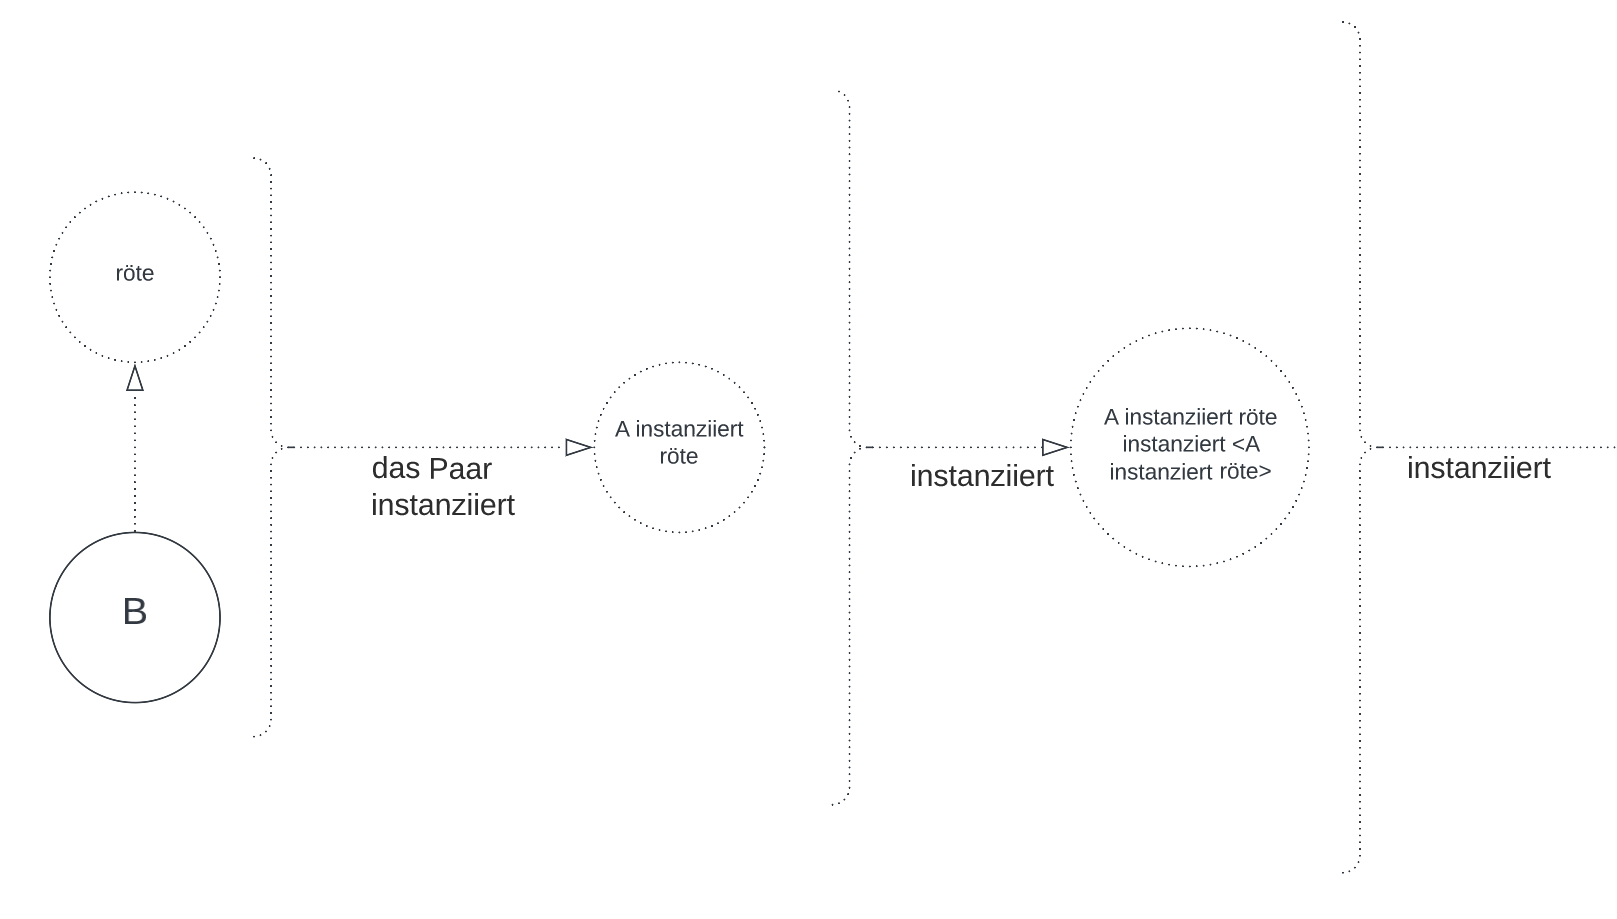
\includegraphics[width=.8\linewidth]{images/infiniter_regress_universalienrealismus.png}
          }
    	\end{minipage}
\end{enumerate}

\paragraph{Einwände}
\begin{enumerate}
	\item Vorwurf der \textit{mysteriösen Natur} der Universalien.
\end{enumerate}

\section{Klassischer Nominalismus I: Tropentheorie}
Der klassische Nominalismus versucht Erklärungen für die qualitative Identiät von Substanzen zu finden, ohne auf Universalien zurückzugreifen. Die (moderate) Variante des klassischen Nominalismus ist die Tropentheorie (D. C. Williams, K. Campell, u.a.).

\paragraph{These} 
\begin{enumerate}[label=(\alph*)]
	\item Es gibt Substanzen (= Einzeldinge), die Eigenschaften instanziieren, aber selbst nicht instanziiert werden können
	\item Es gibt Tropen (= Eigenschaften), die von genau einer Substanz instanziert werden können (bzw. n-stellige Relationen, die genau von einem n-Tubel von Substanzen instanziert werden klönnen).
	\item Dass zwei Substanzen in einer Hinsicht gleich (qualitativ identisch) sind, kann dadurch erklärt werden, dass sie qualitativ identische Tropen instanziieren. 
\end{enumerate}

{\centering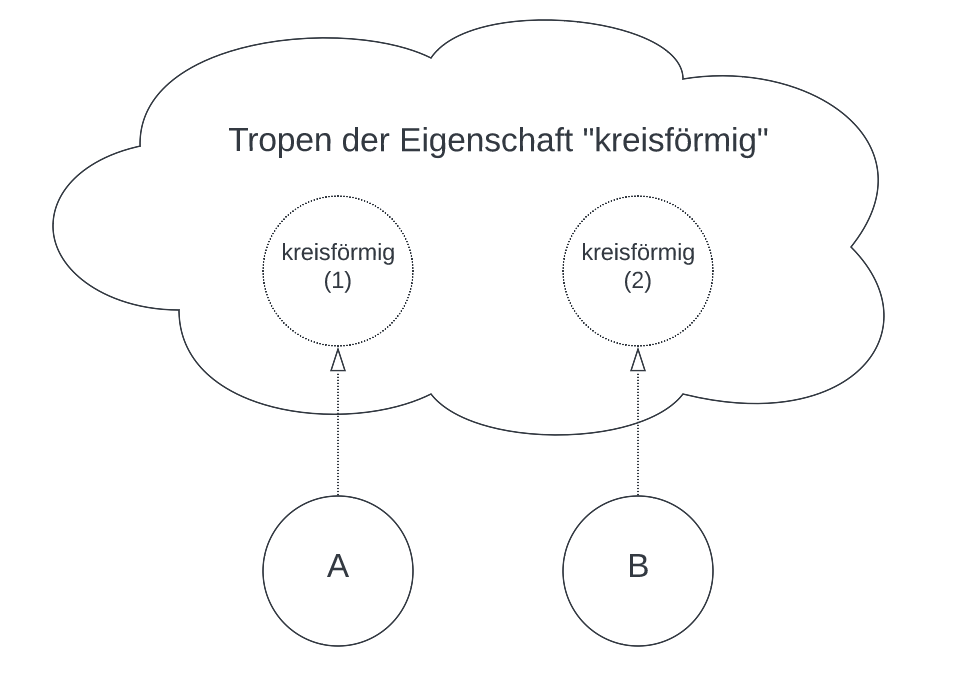
\includegraphics[height=7cm]{images/tropen_uebersicht.png}\endcenter}

\paragraph{Probleme}
\begin{enumerate}
	\item Die Tropentheorie ist (gemäss Ockhams Rasiermesser) nicht sparsamer als die Universalientheorie.
	\item Auch ist der Vorwurf der \textit{mysteriösen Natur} von Universalien ebenso auf Tropen anwendbar. 
	\item Die Tropentheorie erklärt die qualitative Identität von Substanzen durch die qualitative Identität von Tropen, die von den Substanzen instanziiert werden. Es ist aber offen, inwiefern sich die qualitative Identitäten von Tropen vergleichbar sind. Es scheint, als würde sich das gleiche Problem nochmals auftun. 
\end{enumerate}

\section{Klassischer Nominalismus II: Prädikatennominalismus und Konzeptualismus}
\paragraph{These} Zwei numerisch verschiedene Substanzen sind gleich (qualitativ identisch), wenn auf beide das gleiche Prädikat (sprachliche Ausdrücke wie <<ist rot>> oder <<ist ein Mensch>>) zutrifft.
\paragraph{Erklärung} Der Prädikatennominalismus kommt ohne Tropen oder Universalien aus und interpretiert <<Nominalismus>> im Wortsinn. Er schaut dabei die Prädikate an, also die Ausdrücke, die sagen, was in einem Satz <<passiert>>. Für den Satz <<Er ist gross>> wäre das Prädikat <<ist gross>>; Es verlinkt das Subjekt des Satzes mit einer (wahrheitsfähigen) Eigenschaft. 

\vspace{10pt}
{\centering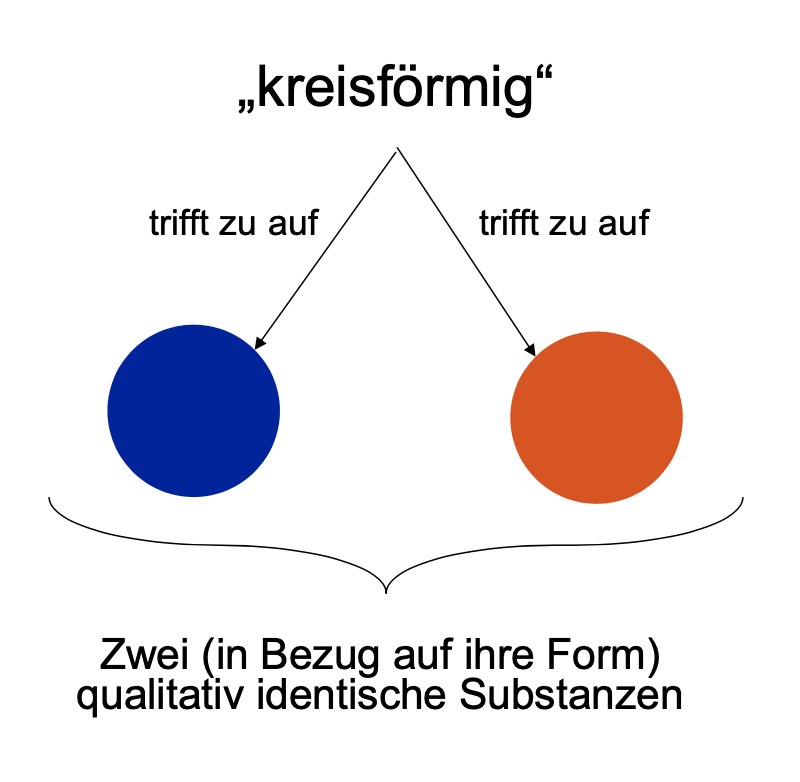
\includegraphics[height=7cm]{images/praedikatennominalismus.png}\endcenter}

\paragraph{Argumente}
\begin{enumerate}
	\item Universalienrealisten, Tropentheoretiker und Prädikatennominalisten sagen, dass Prädikate \textit{existieren}, ebenso wie Substanzen, auf die diese Prädikate zutreffen. Die anderen benötigen aber noch zusätzliche Entitäten!
	\item Während andere Theorien (z.B. Universalienrealismus, Tropentheorie) andere Entitäten (z.B. Universalien oder Tropen) benötigen, kommt der Prädikatennominalismus ohne neu postulierte Entitäten aus.  
	\item Gemäss Ockhams Rasiermesser ist diese Theorie zu bevorzugen, da sie am sparsamsten ist. 
\end{enumerate}
\paragraph{Einwände}
\begin{enumerate}
	\item Es ist unklar, was Prädikatennomalisten mit <<ist kreisförmig>> meinen. Der Ausdrück könnte einem bestimmten Gegenstand (Token) eine Eigenschaft zuweisen, ebenso wie die Kategorie von allen kreisförmigen Gegenständen meinen (Typ). Der Prädikatennominalist sagt dazu, dass es sich entweder um einen Typ handelt oder um ein Vorkommnis eines bestimmten Types. Aber selbst dann ist fragwürdig, was es genau ausmacht, dass verschiedene Vorkommnisse zu einem bestimmten Typ zugeordnet werden können. 
	\item Da wir ständig neue Dinge und Eigenschaften entdecken und somit ständig neue Prädikate der Liste aller Prädikate hinzufügen, bricht das den Prädikatennominalismus, denn Dinge sind so, \textit{weil} sie dasselbe Prädikat haben. Oder in anderen Worten: Prädikate sind nicht durch Eigenschaften von Objekten begründet, sondern Eigenschaften sind durch Prädikate begründet (es gibt Prädikate zuerst, dann die Eigenschaften). 
	\item Intuitiv ist etwas so, wie es ist (z.B. kreisförmig), weil es kreisförmig ist, nicht (!), weil es das Prädikat (<<ist kreisförmig>>) darauf zutrifft. D.h. die Erklärungsrichtung ist kontraintuitiv. 
\end{enumerate}

\subsection{Konzeptualismus}
\paragraph{These} Zwei dinge sind qualitativ identisch, wenn sie unter denselben Begriff fallen.
\paragraph{Erklärung} Der Konzeptualismus besagt, dass etwas kreisförmig ist, weill es unter den Begriff der Kreisförmigkeit fällt. Er ist somit weitgehend analog (wie seine Probleme/Einwände) zum Prädikatennominalismus, bis auf den Unterschied, dass statt sprachlichen Ausdrücken auf \textit{Begriffe} Bezug (Begriff = mentale Entitäten, Komponenten von Gedanken) genommen wird.

\section{Klassischer Nominalismus III: Klassennominalismus}
\paragraph{These} Dass zwei numerisch verschiedene Dinge in einer Hinsicht gleich (qualitativ identisch) sind, kann dadurch erklärt werden, dass beide Dinge zu derselben Klasse gehören, also Elemente derselben Klasse sind.
\paragraph{Erklärung} Der Klassennominalismus benötigt keine Tropen oder Universalien. Er besagt lediglich, dass Eigenschaften durch die Klassenzugehörigkeit von Dingen geschaffen werden. 
\paragraph{Problem}
\begin{enumerate}
	\item Er scheint plausiebel zu sein, bis man bedenkt, dass es Klassen gibt, die nicht heterogen sind, also aus komplett verschiedenen Dingen bestehen und somit in keiner Weise qualitativ identisch sind. Z.B. die Menge aus den Dingen, die ich gerade genannt habe, also \{Eiffelturm, 23, Uranus\}. Nur weil zwei Dinge in die gleiche Klasse gehören, impliziert das nicht Gleichheit. 
\end{enumerate}

\subsection{Klassennominalismus mit natürlichen Klassen}
\paragraph{These} Dass zwei numerisch verschiedene Dinge in einer Hinsicht gleich (qualitativ identisch) sind, kann dadurch erklärt werden, dass beide Dinge zu derselben \textit{natürlichen} Klasse gehören. 
\paragraph{Erklärung} Aus dem Problem für den klassischen Klassennominalismus entsteht der Klassennominalismus mit natürlichen Klassen. 

Was genau natürliche Klassen sind, ist (gemäss Armstrong) den Naturwissenschaften und ihren besten Theorien überlassen. Es kann jedoch nach \textit{Natürlichkeit} unterschieden werden. Z.B. ist die Klasse der farbigen Dinge weniger natürlich (homogen), als die Klasse mit den orangen Dingen. 

\paragraph{Einwände}
\begin{enumerate}
	\item Wenn zwei Klassen mit exakt denselben Dingen existieren, so wären diese Klassen ja gleich. Dies ist wäre (angenommen) der Fall, wäre bei der Klasse aller Tiere mit Nieren und der Klasse aller Tiere mit Herz. Somit wären, obwohl wir hier von verschiedenen Eigenschaften sprechen, diese exakt gleich (man müsste nicht mehr sagen, dass etwas Nieren hat, wenn man sagt, dass es ein Herz hat). Das ist aber absurd!
	\item Es ist gegen die Intuition, weil die Erklärung verkehrt ist. Etwas ist kreisförmig, weil es kreisförmig ist, nicht: Es gehört zur Klasse Kreisförmig und deswegen ist es kreisförmig. 
\end{enumerate}

\section{Radikaler Nominalismus (ostrich nominalism}
\paragraph{These} Etwas hat eine Eigenschaft, weil es diese Eigenschaft hat
\paragraph{Erklärung} Der radikale Nominalismus macht es sich leicht. Er besagt, dass etwas so ist, weil es eben so ist. Er geht davon aus, dass Eigenschaften \textit{primitive} Wahrheiten sind, also nicht weiter erklärbar. Das heisst auch, dass er auf die Frage, inwiefern Dinge identisch sind, nur mit <<Es ist einfach so>> antworten kann. 

Er ist jedoch klar vom Prädikatennominalismus zu unterscheiden, da er bestreitet, dass es eine abstrakte Universale oder Trope der Kreisförmigkeit gibt. 
\paragraph{Einwände}
\begin{enumerate}
	\item Es ist schwierig Dinge wie <<Rot ist eine Farbe>> oder <<Es gibt Rot im Sinne von Rot-Sein>> mit dem radikalen Nominalismus zu erklären. 
		
		\textbf{Quinte's Antwort}: Es gäbe den Umweg der Paraphrasen. Also Umformulierungen, die nicht logisch implizieren, dass Rot-Sein existiert. Bsp. <<Rot ist eine Farbe>> --> <<Alle roten Dinge sind farbig>>. Es ist aber äusserst schwierig, dies für alle Ausdrücke zu machen und zusätzlich ist es fragwürdig, ob diese Paraphrasen auch wirklich denselben Aussagengehalt haben. 
\end{enumerate}

\end{document}